\documentclass[fleqn,12pt]{article}

\usepackage[margin=15mm]{geometry}
\usepackage[utf8]{inputenc}
\usepackage[bulgarian]{babel}
\usepackage[unicode]{hyperref}
\usepackage{amsfonts}
\usepackage{amssymb}
\usepackage{enumitem, hyperref}
\usepackage{upgreek}
\usepackage{graphicx}
\usepackage{mathtools}
\usepackage{graphicx}
\graphicspath{ {./images/} }

\setcounter{secnumdepth}{5}
\setcounter{tocdepth}{5}

\makeatletter
\newcommand\subsubsubsection{\@startsection{paragraph}{4}{\z@}{-2.5ex\@plus -1ex \@minus -.25ex}{1.25ex \@plus .25ex}{\normalfont\normalsize\bfseries}}
\newcommand\subsubsubsubsection{\@startsection{subparagraph}{5}{\z@}{-2.5ex\@plus -1ex \@minus -.25ex}{1.25ex \@plus .25ex}{\normalfont\normalsize\bfseries}}
\makeatother


\title{Oпределен  интеграл.  Дефиниция  и  свойства.  Интегруемост  на непрекъснати функции. Теорема на Нютон-Лайбниц}
\author{v1.0}
\date{16 юни 2021}

\begin{document}

\maketitle

\tableofcontents
\pagebreak

\begin{flushleft}

\section{Разбиване на интервал}

\subsection{Дефиниция на разбиване на интервал}
Разбиване $\tau$ на интервала $[a,b]$ наричаме системата от точки $\{x_i\}_{i=0}^n : а = x_0 < x_1 < ... < x_n = b$. В следствие от разбиването
се образуват n непрепокриващи се подинтервала на $[a,b] : [a, x_1], [x_1, x_2], ... [x_{n-1}, b]$, като дължината на интервал $i \in [1,n]$ е $\Delta_i = x_i - x_{i-1}$.

\subsection{Разбиване съдържащо друго разбиване}
Нека $x,y$ са две разбивания на интервала $[a,b]$, съответно на системите от точки $\{x_i\}_{i=0}^{n}$ и  $\{y_i\}_{i=0}^{m}$. Казваме че разбиването $y$ съдържа в себе си разбиването $x$ ($x \prec y$), ако
$\{x_i\}_{i=0}^{n} \subseteq  \{y_i\}_{i=0}^{m}, n \leq m$.

\subsection{Междинни точки на разбиване}
Нека $\tau$ e разбиване на интервала $[a,b]$. Тогава точките $\{\xi_i\}_{i=1}^n : \xi_i \in [x_{i-1},x_i]$ ще наричаме междинни точки на това разбиване.

\subsection{Диаметър на разбиване}
Диаметър на разбиването $\tau$ дефинираме дължината на най-дългият интервал, който се образува от разбиването, т.е $d(\tau)=max_{i\in[1,n]} \Delta_i$.

\section{Интегруемост по Риман}
\subsection{Дефиниция на Риманова сума}
Римановата сума на функцията $f(x)$, съответстваща на разбиването $\tau$ на интервала [a,b] и на избраните междинни точки $\{\xi_i\}_{i=1}^n$, се определя от формулата: 
$R(f;\tau;\{\xi_i\})=\sum_{n = 1}^{n} f(\xi)(x_i-x_{i-1})$.  

\subsection{Риманов интеграл}
Стойността $I$ наричаме граница на римановите суми $R_\tau(f)$ на функцията $f$ при $d(\tau)\rightarrow0$, ако $\forall\epsilon>0, \exists \delta>0 :$ за всяко разбиване $\tau$
на интервала $[a,b]$ с $d(\tau)<\delta$ е изпълнено че $|R_f(x) - I|<\epsilon$ (при произволен избор на междинни точки). Всяка функцията $f$, за която съществува такава граница на римановите суми в $[a,b]$,
се нарича интегруема (по Риман) в $[a,b]$, a границата $I$ се нарича определен интеграл от $f$ в интервала $[a,b]$ и се бележи с $I = \int_{a}^{b}  f(x)\,dx$ 

\subsection{Всяка интегруема по Риман функция е ограничена}
\textbf{Доказателство: } Нека функцията $f$ e интегруема по Риман в интервала $[a,b]$ и $I = \int_{a}^{b}  f(x)\,dx$. Нека изберем $\epsilon=1$ тогава $\exists \delta>0$, такова че 
за всяко разбиване $\tau$ на интервала $[a,b]$ с $d(\tau)<\delta$ е изпълнено че $|R_\tau(f) - I|<1$, т.е $I-1<R_f(x)<I+1$. От което следва, че множеството от римановите суми на функцията
$f$ е ограничено когато $d(\tau)<\delta$. Остава да докажем, че $f$ е ограничена в интервала $[a,b]$.
Да допуснем че $f$ не е ограничена в $[a,b]$. Тогава съществува поне един интервал от разбиването $\tau$, в който $f$ е неограничена - нека такъв интервал е например $[x_{j-1},x_j]$.
Нека в този интервал вземем редица от точки $\{\xi_j^{(k)}\}_k : |f(\xi_j^{(k)})| > k, \forall k \in [0,\infty]$, следователно $\lim_{k \rightarrow +\infty} f(\xi_j^{(k)}) = +\infty$.
Нека за останите интервали фиксираме прозиволни междинни точки $\{\xi_i\}_{i=1,i \neq j}^n : \xi_i \in [x_{i-1},x_i]$ и тогава $\sum_{i=1,i \neq j}^{n} f(\xi_i)(x_i - x_{i-1})$ е с фиксирана стойност.\\
Добавяйки към тази сума събираемото $f(\xi_j^{(k)})(x_j - x_{j-1})$ получаваме римановата сума на $f$ в $[a,b]$:\\
$R(f;\tau;\xi_1,\xi_2, ... ,\xi_{j-1},\xi_j^{(k)},\xi_{j+1}, ... ,\xi_n)$. Тогава е изпълнено, че:\\
$\lim_{x \rightarrow \infty} R(f;\tau;\xi_1,\xi_2, .. ,\xi_{j-1},\xi_j^{(k)},\xi_{j+1}, ... ,\xi_n) = \lim_{x \rightarrow \infty} (f(\xi_j^{(k)})(x_j - x_{j-1}) + \sum_{i=1,i \neq j}^{n} f(\xi_i)(x_i - x_{i-1})) = +\infty$ \\
Което означава че множеството от риманови суми на $f$ в $[a,b]$ е неограничено, включително когато $d(\tau)<\delta$. Следователно противоречие с допускането, че $f$ e неограничена в $[a,b]$.
Теоремата е доказана. 

\section{Интегруемост по Дарбу}
\subsection{Малка сума на Дарбу}
Нека $f$ е ограничена в интервала $[a,b]$ и $\tau$ е разбиване на интервала $[a,b]$ на системата от точки $\{x_i\}_{i=0}^{n}$.
Тогава "малка сума на Дарбу" дефинираме като $\underline{s}(f,[a,b],\tau)=\sum_{i=1}^{n} m_i(x_i-x_{i-1})$, където $m_i=\inf_{x\in[x_{i-1},x_i]}f(x)$.

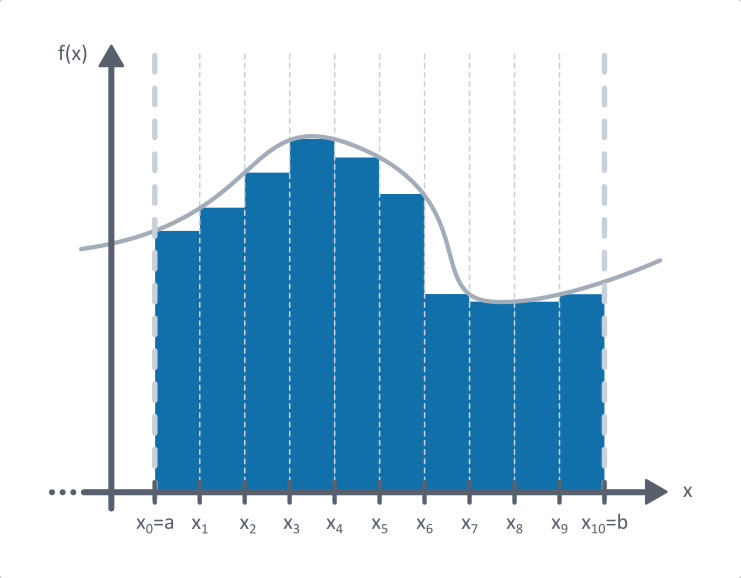
\includegraphics{darboux_lower_sum.png}


\subsection{Голяма сума на Дарбу}
Нека $f$ е ограничена в интервала $[a,b]$ и $\tau$ е разбиване на интервала $[a,b]$ на системата от точки $\{x_i\}_{i=0}^{n}$.
Тогава "голяма сума на Дарбу" дефинираме като $\overline{S}(f,[a,b],\tau)=\sum_{i=1}^{n} M_i(x_i-x_{i-1})$, където $M_i=\sup_{x\in[x_{i-1},x_i]}f(x)$.

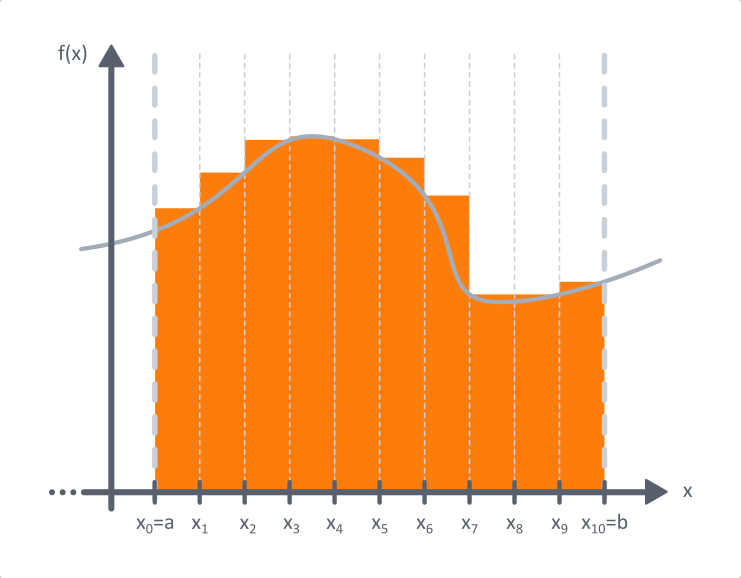
\includegraphics{darboux_higher_sums.png}

\subsection{Характеристики на сумите на Дарбу}
\subsubsection{Връзка между сумите на Дарбу и Римановите суми}
Нека $f$ e интегруема по Риман в интервала $[a,b]$ и $\tau$ е разбиване на интервала $[a,b]$ на системата от точки $\{x_i\}_{i=0}^{n}$. Toгава е в сила, че:\\
$\underline{s}(f,[a,b],\tau) \leq R_f(\tau) \leq \overline{S}(f,[a,b],\tau)$

\subsubsection{Свойство 1: Малките суми нарастват, а не намаляват}
Нека $x,y$ са разбивания на интервала $[a,b]$, такива че разбиването $y$ строго съдържа в себе си разбиването $x$. Тогава е в сила, че:
$underline{s}(f,[a,b],x) < underline{s}(f,[a,b],y)$\\
\textbf{Доказателство: } Нека системата от точки на разбиването $y$ съдържа точно една точка в повече от системата от точки на разбиването $x$.
Нека тази точка е $x^{*} \in [x_{j-1},x_j], j\in [0,n]$. Нека разгледаме израза:
$\underline{s}(f,[a,b],y)-\underline{s}(f,[a,b],x) = (m_1(x^{*} - x_{j-1}) + m_2(x_j - x^{*}) + \sum_{i=0,i \neq j}^{n} m_i(x_i - x_{i-1})) - (\sum_{i=0}^{n} m_i(x_i - x_{i-1}))$,\\ kъдето
$m_1 =\inf_{x\in[x_{j-1},x^{*}]}f(x), m_2 =\inf_{x\in[x^{*},x_j]}f(x)$.\\
$\underline{s}(f,[a,b],y) - \underline{s}(f,[a,b],x) = m_1(x^{*} - x_{j-1}) + m_2(x_j - x^{*}) - m_j(x_j - x_{j-1}) = m_1(x^{*} - x_{j-1}) + m_2(x_j - x^{*}) - m_j(x_j + x^{*} - x^{*} - x_{j-1})$
$ = (m_1-m_j)(x^{*} - x_{j-1}) + (m_2-m_j)(x_j - x^{*})$. Но понеже $m_1 \geq m_j, m_2 \geq m_j$ понеже $m_1,m_2$ са минимумите на $f$ в подинтервали на $[x_{j-1},x_j]$.
Следователно $\underline{s}(f,[a,b],y) - \underline{s}(f,[a,b],x) = (m_1-m_j)(x^{*} - x_{j-1}) + (m_2-m_j)(x_j - x^{*}) \geq 0$.

\subsubsection{Свойство 2: Големите суми намаляват, а не нарастват}
Нека $x,y$ са разбивания на интервала $[a,b]$, такива че разбиването $y$ строго съдържа в себе си разбиването $x$. Тогава е в сила, че:
$\overline{S}(f,[a,b],y) < \overline{S}(f,[a,b],x)$\\
\textbf{Доказателство: } Нека системата от точки на разбиването $y$ съдържа точно една точка в повече от системата от точки на разбиването $x$.
Нека тази точка е $x^{*} \in [x_{j-1},x_j], j\in [0,n]$. Нека разгледаме израза:
$\overline{S}(f,[a,b],y) - \overline{S}(f,[a,b],x) = (M_1(x^{*} - x_{j-1}) + M_2(x_j - x^{*}) + \sum_{i=0,i \neq j}^{n} M_i(x_i - x_{i-1})) - (\sum_{i=0}^{n} M_i(x_i - x_{i-1}))$,\\ kъдето
$M_1 =\sup_{x\in[x_{j-1},x^{*}]}f(x), M_2 =\sup_{x\in[x^{*},x_j]}f(x)$.\\
$\overline{S}(f,[a,b],y) - \overline{S}(f,[a,b],x) = M_1(x^{*} - x_{j-1}) + M_2(x_j - x^{*}) - m_j(x_j - x_{j-1}) = M_1(x^{*} - x_{j-1}) + M_2(x_j - x^{*}) - M_j(x_j + x^{*} - x^{*} - x_{j-1})$
$ = (M_1-M_j)(x^{*} - x_{j-1}) + (M_2-M_j)(x_j - x^{*})$. Но понеже $M_1 \leq M_j, M_2 \leq M_j$ понеже $M_1,M_2$ са максимумите на $f$ в подинтервали на $[x_{j-1},x_j]$.
Следователно $\overline{S}(f,[a,b],y) - \overline{S}(f,[a,b],x) = (M_1-M_j)(x^{*} - x_{j-1}) + (M_2-M_j)(x_j - x^{*}) \leq 0$.

\subsubsection{Свойство 3: Всяка малка сума на Дарбу е по-малка или равна на всяка голяма}
\textbf{Доказателство: }
Нека $f$ e ограничена в интервала $[a,b]$ и $x,y$ са произволни разбивания на интервала $[a,b]$. Нека $z$ е също разбиване на интервала $[a,b]$,
съдържащо в себе си разбиванията $x,y$ ($x \preceq z, y \preceq z$). Тогава :
от свойство 1 следва, че $\underline{s}(f,[a,b],x) \leq \underline{s}(f,[a,b],z)$
от свойство 2 следва, че $\overline{S}(f,[a,b],z) \leq \overline{S}(f,[a,b],y)$
Следователно $\underline{s}(f,[a,b],x) \leq \underline{s}(f,[a,b],z) \leq \overline{S}(f,[a,b],z) \leq \overline{S}(f,[a,b],y)$.\\
Понеже избрахме $x,y$ да са произволни разбивания на $[a,b]$, то твърдението е изпълнено. 

\subsection{Интегруемост по Дарбу}
От Свойство 3 на сумите на Дарбу знаем, че всяка малка сума на Дарбу е по-малка или равна на всяка голяма, т.е малките суми на Дарбу имат горна граница, а горните суми на Дарби долна граница.
Нека дефинираме $\underline{I}=\inf_\tau \underline{s}(f,[a,b],\tau)$ и $\overline{I}=\sup_\tau \overline{S}(f,[a,b],\tau)$,
тогава $\underline{I}$ и  $\overline{I}$ наричаме съответно долен и горен интеграл на Дарбу. Ако $\underline{I}=\overline{I}=I$, то функцията $f$ е интегруема по Дарбу в интервала $[a,b]$.

\section{Теорема: Връзка между интегруемост по Риман и по Дарбу}
Една функция е интегруема по дефиницията на Риман, т.т.к е интегруема по дефиницията на Дарбу. При това и двете дефиниции дават една и съща стойност на интеграла.
(Понеже доказателството на тази теорема изисква доказателстовот на 3-4 леми/свойства и не се изисква от конспекта, то ще използваме на готово теоремата.)

\section{Дадена функция е интегруема по Риман тогава и само тогава, когато $\forall\epsilon > 0$ съществуват голяма и малка сума на Дарбу $\overline{S}$ и $\underline{s}$ такива, че $\overline{S}-\underline{s} < \epsilon$}
\textbf{Доказателство ($\Longrightarrow$):} Нека $f$ e интегруема по Риман в $[a,b]$, следователно е интегруема по Дарбу в $[a,b]$. \\
Ще докажем че $\forall\epsilon > 0$ съществуват голяма и малка сума на Дарбу $\overline{S}$ и $\underline{s}$ такива, че $\overline{S} - \underline{s} < \epsilon$.
Тогава $\underline{I}=\overline{I}=I$ и нека изберем произволно $\epsilon > 0$. Понеже $I$ е горна граница на малките суми на Дарбу, то 
$I - \frac{\epsilon}{2}$ не е горна граница на малките суми на Дарбу. Понеже $I$ е долна граница на големите суми на Дарбу, то $I + \frac{\epsilon}{2}$ не е долна граница на големите суми на Дарбу.
Следователно $\exists \tau_1,\tau_2$ разбивания на интервала $[a,b]$, такива че: \\
$I - \frac{\epsilon}{2} < \underline{s}(f,[a,b],\tau_1) \leq I$
$I \leq \overline{S}(f,[a,b],\tau_2) < I + \frac{\epsilon}{2}$
Нека $\tau_3$ съдържа в себе си разбиванията $\tau_1,\tau_2$. Toгава от Свойство 3 на сумите на Дарбу е изпълнено, че :\\
$I - \frac{\epsilon}{2} < \underline{s}(f,[a,b],\tau_1) \leq  \underline{s}(f,[a,b],\tau_3) \leq I \leq \overline{S}(f,[a,b],\tau_3) \leq \overline{S}(f,[a,b],\tau_2) < I + \frac{\epsilon}{2}$
$\overline{S}(f,[a,b],\tau_3) - \underline{s}(f,[a,b],\tau_3) < I + \frac{\epsilon}{2} - I + \frac{\epsilon}{2} = \epsilon$
Следователно твърденуето в тази посока е в сила.
\textbf{Доказателство ($\Longleftarrow$):}
Нека $f$ e ограничена функция в $[a,b]$ за която е изпълнено,че $\forall\epsilon > 0$ съществуват голяма и малка сума на Дарбу $\overline{S}$ и $\underline{s}$ такива, че $\overline{S} - \underline{s} < \epsilon$.
Ще докажем, че $f$ e интегруема по Риман в $[a,b]$. Нека приемем, че $f$ не е интегруема по Риман, следователно не е интегруема по Дарбу - т.е $\underline{I} < \overline{I}$.
Нека $\epsilon = \frac{\underline{I} + \overline{I}}{2}$, тогава $\exists\tau : \overline{S}(f,[a,b],\tau) - \underline{s}(f,[a,b],\tau) < \epsilon$.
Понеже $\underline{s}(f,[a,b],\tau) \leq \underline{I} < \overline{I} \leq \overline{S}(f,[a,b],\tau) \Longrightarrow \epsilon > \overline{S}(f,[a,b],\tau) - \underline{s}(f,[a,b],\tau) \leq \overline{I} - \underline{I} = 2\epsilon$
Следователно е в сила, че $\epsilon > 2\epsilon \Leftrightarrow \epsilon < 0$.
Противоречие с допускането че $\epsilon>0 \Longrightarrow \underline{I}=\overline{I}$, от което следва интегруемост на $f$ по Дарбу, а и съответно по Риман, в интервала $[a,b]$.

\section{Равномерна непрекъснатост}

\subsection{Дефиниция на равномерна непрекъснатост}
Казваме че функцията $f$ e равномерно непрекъсната в интервала $D$, ако $\forall \epsilon>0, \exists \delta>0 : |x_1 - x_2|<\delta, x_1,x_2 \in D \Longrightarrow |f(x_1)-f(x_2)|<\epsilon$

\subsection{Теорема на Кантор: Връзка между непрекъснатост и равномерна непрекъснатост}
Ако функцията $f$ е непрекъсната в краен и затворен интервал, то тя е равномерно непрекъсната в този интервал.

\subsection{Дефинция на осцилация}
Нека $f$ е непрекъсната функция в интервала $[a,b$]. Числото $\omega(f,D) = \sup_{x \in D} f(x)$ се нарича осцилация на функцията $f$ в интервалa $D$.

\subsection{Връзка между равномерната непрекъснатост и осцилацията на функция}
Казваме че функцията $f$ e равномерно непрекъсната в интервала $D$, ако $\forall \epsilon>0, \exists \delta>0 :$ за всеки подинтервал $D_i: \Delta_{D_i} < \delta$ е изпълнено, че $\omega(f,D_i \cap D) < \epsilon$.

\subsection{Следствие: Теорема за осцилацията}
Ако $f:[a,b]->R$ е непрекъсната в крайния и затворен интервал $[a,b]$, то $\forall \epsilon>0$ интервалът може да се раздели на краен брой непресичащи се интервали $D_i, i\in[0,k]$,
такива че осцилацията на $f$ ($\omega(f,D_i)$) във всеки един от тях е по-малка от $\epsilon$. 


\section{Всяка непрекъсната функция в краен и затворен интервал е интегруема по Риман}
\textbf{Доказателство :} Нека функцията $f$ е непрекъсната в интервала $[a,b]$. Нека $\epsilon > 0$ и от Теоремата на Кантор и от Теоремата за осцилацията следва, че $\exists \delta>0 :$ осцилация на  $f$ във всеки подтинтервал
на $[a,b]$ с дължина по-малка $\delta$ да е $\frac{\epsilon}{2(b-a)}$, т.е $\forall x_1,x_2 \in [a,b] , |x_1 - x_2| < \delta$ е изпълнено $|f(x_1)-f(x_2)| < \frac{\epsilon}{2(b-a)}$.
Нека имаме разбиване $\tau: d(\tau)<\delta$ на интервала $[a,b]$ на системата от точки $\{x_i\}_{i=0}^{n}$ и нека следния израз:
$\overline{S}(f,[a,b],\tau) - \underline{s}(f,[a,b],\tau) = \sum_{i=1}^{n} (M_i - m_i)(x_i - x_{i-1})$,\\
но $M_i - m_i$ е точно осцилацията на $f$ в интервала $[x_{i-1},x_i]$.\\
Следователно $\overline{S}(f,[a,b],\tau) - \underline{s}(f,[a,b],\tau) < \frac{\epsilon}{2(b-a)}\sum_{i=1}^{n} (x_i - x_{i-1}) = \frac{\epsilon}{2(b-a)}(b-a)< \epsilon$.\\
От това следва, че $f$ e интегруема по Риман в интервала $[a,b]$.

\section{Основни свойства на Римановия интеграл}
Нека $f(x),g(x)$ са интегруеми в интервала $[a,b]$. Тогава важат следните свойства:
\begin{enumerate}
    \item $\int_{a}^{b}  f(x)\,dx = -\int_{b}^{a} f(x)\,dx$
    \item $\int_{a}^{a}  f(x)\,dx = 0$
    \item $\int_{a}^{b}  f(x)\,dx = \int_{a}^{b}  f(t)\,dt$
    \item ако $c\in[a,b]$, то е изпълнено, че $\int_{a}^{c} f(x)\,dx + \int_{c}^{b} f(x)\,dx = \int_{a}^{b} f(x)\,dx$
    \item ако $f(x)\geq 0, x \in [a,b] \Rightarrow \int_{a}^{b}  f(x)\,dx \geq 0$
    \item ako $a < b$ и $f(x) \leq g(x), x \in [a,b] \Rightarrow \int_{a}^{b}  f(x)\,dx \leq \int_{a}^{b}  g(x)\,dx$
    \item $(f(x) + g(x))$ и $\lambda f(x), \lambda = const$ също са интегруеми, като $\int_{а}^{b} \lambda f(x)\,dx = \lambda \int_{а}^{b} f(x)\,dx$ и $\int_{а}^{b} g(x)\,dx + \int_{a}^{b} f(x)\,dx = \int_{а}^{b} (f(x)+g(x))\,dx$
    \item понеже функцията $f(x)$ е интегруема в $[a,b]$, то $|f(x)|$ също е интегруема в $[a,b]$ и $|\int_{a}^{b} f(x)\,dx| \leq \int_{a}^{b}  |f(x)|\,dx$
    \item ако $\exists M,m \in R:$ за всяко $x \in [a,b]$ е изпълнено $m \leq f(x) \leq M$, то е изпълнено че $m(b-a) \leq \int_{a}^{b} f(x) \leq M(b-a)$
\end{enumerate}

\section{Теорема за средните стойности}
\subsection{Теорема на Болцано}
Ако $f$ e непрекъсната в $[a,b]$ и $f(a)f(b)<0$, то $\exists c \in (a,b): f(c) = 0$

\subsection{Следствие от Теорема на Болцано}
Всяка непрекъсната функция $f$ в $[a,b]$ приема всички стойности от минимума $m$ и максимума си $M$ в този интервал.

\subsection{Теорема за средните стойности}
Ако функцията $f$ е непрекъсната в $[a,b]$, тогава съществува поне една точка $c \in [a,b]: f(c)(b-a) = \int_{a}^{b}  f(x)\,dx$.
\textbf{Доказателство :} Ако $f$ е непрекъсната, то от теоремата на Вайерщрас следва, че $m \leq f(x) \leq M: m = \inf_{x \in [a,b]}f(x), M = \sup_{x \in [a,b]}f(x)$.
Понеже $f$ е непрекъсната в $[a,b]$, то $f$ e интегруема в $[a,b]$ и от Свойство 9 на Римановите интеграли следва, че $m(b-а) \leq \int_{a}^{b}  f(x)\,dx \leq M(b-a)$.\\
$m \leq \frac{\int_{a}^{b} f(x)\,dx}{b-a} \leq M$. От следстивето от теоремата на Болцано следва, че $\exists c \in [a,b]: f(c) = \frac{\int_{a}^{b} f(x)\,dx}{b-a}$.
С това доказателството е завършено.

\section{Теорема на Лайбниц-Нютон}
\subsection{Теорема на Лайбниц-Нютон}
Нека $f$ е непрекъсната в $[a,b]$ и $F(x)=\int_{a}^{x} f(t)\,dt$. Тогава $F(x)$ е диференцируема в $[a,b]$ и $\forall x \in [a,b], F'(x)=f(x)$ ($F(x)$ е примитивна на $f(x)$ в $[a,b]$).
\textbf{Доказателство :} Нека $f$ е непрекъсната в $[a,b]$, тогава $f$ е непрекъсната в $[a,x], x \in [a,b]$. Понеже  $f$ е непрекъсната в $[a,x]$, то $f$ е интегруема в $[a,x]$.
Нека дефинираме $F(x)=\int_{a}^{x} f(t)\,dt$ и нека вземем числото $h: x+h\in[a,b]$. Да разгледаме диференчното частно $\frac{F(x+h)-F(x)}{h}$.
$\frac{F(x+h)-F(x)}{h} = \frac{\int_{a}^{x+h} f(t)\,dt - \int_{a}^{x} f(t)\,dt}{h} = \frac{\int_{a}^{x+h} f(t)\,dt + a\int_{x}^{a} f(t)\,dt}{h} = \frac{\int_{x}^{x+h} f(t)\,dt}{h}$
От Теоремата за среднисте стойности следва, че $\exists c \in [x,x+h]: f(c)h = \int_{x}^{x+h} f(t)\,dt$
Следователно $\frac{F(x+h)-F(x)}{h} = f(c)$. Понеже $c \in [x,x+h]$, то при $h \rightarrow 0$ следва, че $c \rightarrow x$.
$F'(x) = \lim_{h \rightarrow 0} \frac{F(x+h)-F(x)}{h} = lim_{h \rightarrow 0} f(c) = f(x)$. Следователно $F'(x)$ е диференцируем в $[a,b]$ и $\forall x \in [a,b] F'(x)=f(x)$.
Теоремата е доказана.

\subsection{Формула на Лайбниц-Нютон (използване на теоремата за изчисляване на определен интеграл)}
Нека $f$ е непрекъсната в $[a,b]$ и $\Phi(x)$ e нейна примитивна в $[a,b]$, т.е $\Phi'(x)=f(x), \forall x \in [a,b]$. Тогава е изпълнено, че
$\int_{a}^{b} f(x)\,dx = \Phi(b) - \Phi(a)$
\textbf{Доказателство :} $f$ е непрекъсната и нека $F(x)=\int_{a}^{x} f(t)\,dt$ . Oт Теоремата на Лайбниц-Нютон следва, че $F'(x)=f(x), \forall x \in [a,b]$.
Тогава $F'(x)=\Phi'(x), \forall x \in [a,b]$ и следователно $F(x) = \Phi(x) + C, C = const$.
Ако $x = a$ то $0 = \int_{a}^{а} f(t)\,dt = F(a) = \Phi(a) + C \Rightarrow C = \Phi(a)$.
Ако $x = b$ то $ \int_{a}^{b} f(t)\,dt = F(b) = \Phi(b) - \Phi(a)$.
С това доказателството е завършено.

\subsection{Пример за прилагане на Формула на Лайбниц-Нютон}
Искаме да решим интегралът $\int_{0}^{5} x\,dx$. $x$ е непрекъсната функция в $[0,5]$ и примитивната й функция $\Phi(x)=\frac{x^2}{2}$.
Следователно използвайки формулата на Лайбниц-Нютон получаваме, че $\int_{0}^{5} x\,dx = \Phi(5) - \Phi(0) = \frac{25}{2} - \frac{0}{2} = 13.5$

\end{flushleft}
\end{document}